\subsubsection{Simulation of the Controllers}
The z translational velocity controller, acting on the non-linear plant with attitude control, is subjected to a step input reference signal in simulation.\\
In \autoref{fig:velocityControllerZ} a step reference of \SI{1}{m s^{-1}} is imposed on the controller. This reveals a rise time of \SI{0.4}{s}, an overshoot of 16.4 $5 \%$ and a settling time of \SI{3}{s}.\\
The control action imposed by the z translational controller is shown in \autoref{fig:velocityControllerZAction}. This is the sum of rotational speeds in the motors which is added to the equilibrium speeds to achieve response in \autoref{fig:velocityControllerZ}.

\begin{minipage}{\linewidth}
    \begin{minipage}{0.45\linewidth}
        \begin{figure}[H]
            \vspace{-.4cm}
            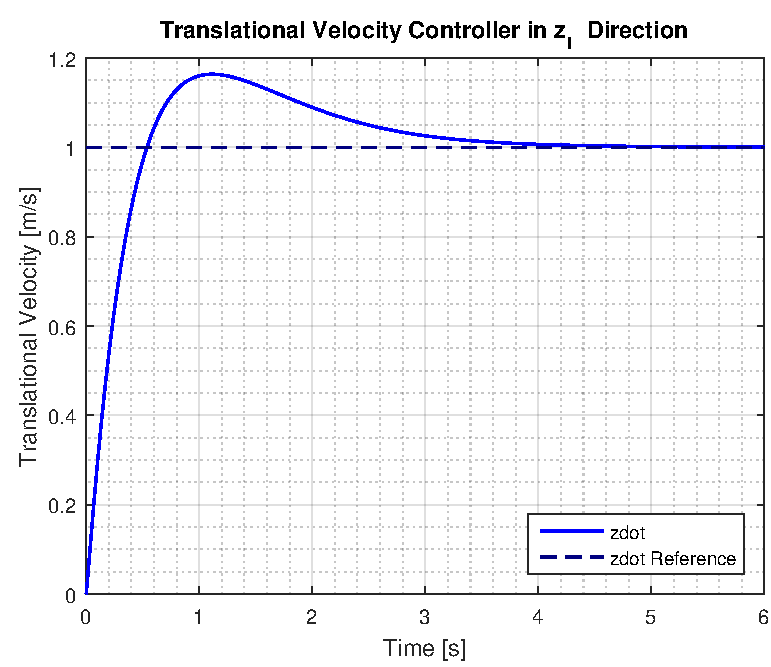
\includegraphics[scale=.45]{figures/velocityControllerZ}
            \centering			
            \captionof{figure}{Step response of the z translational velocity controller.}
            \label{fig:velocityControllerZ}
        \end{figure}
    \end{minipage}
    \hspace{0.03\linewidth}
    \begin{minipage}{0.45\linewidth}
        \begin{figure}[H]
            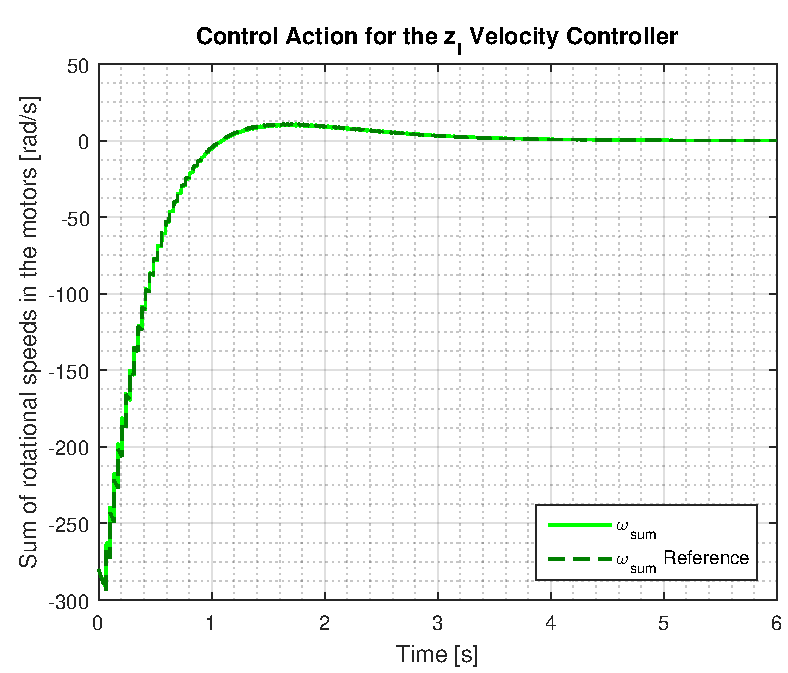
\includegraphics[scale=.45]{figures/velocityControllerZAction}
            \centering
            \captionof{figure}{Control action imposed on the system by the z translational velocity controller to achieve the response in \autoref{fig:velocityControllerZ}.}
            \label{fig:velocityControllerZAction}
        \end{figure}
    \end{minipage}
\end{minipage}

The z translational position controller, acting on the z translational velocity controller, which acts on the non-linear plant with attitude control, is subjected to a step input reference signal in simulation.\\
In \autoref{fig:positionControllersZ} a step reference of \SI{1}{m} is imposed on the controller. This reveals a rise time of \SI{1.278}{s}, an undershoot of  $4.8 \%$ and a settling time of \SI{2.1}{s}. In \autoref{fig:positionControllerZAction} the control action imposed by the z translational position controller is shown. This is the translational velocity, which is denoted zdot Reference in the \autoref{fig:positionControllerZAction}, where zdot is the velocity applied by the velocity controller.

\begin{minipage}{\linewidth}
    \begin{minipage}{0.45\linewidth}
        \begin{figure}[H]
            \vspace{-1.3cm}
            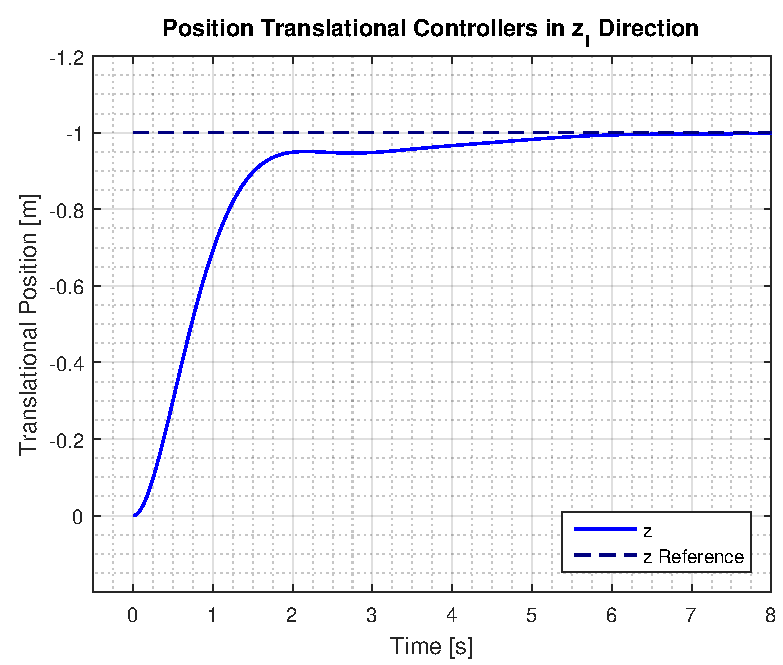
\includegraphics[scale=.45]{figures/positionControllerZ}
            \centering			
            \captionof{figure}{Step response of the z translational position controller.}
            \label{fig:positionControllersZ}
        \end{figure}
    \end{minipage}
    \hspace{0.03\linewidth}
    \begin{minipage}{0.45\linewidth}
        \begin{figure}[H]
            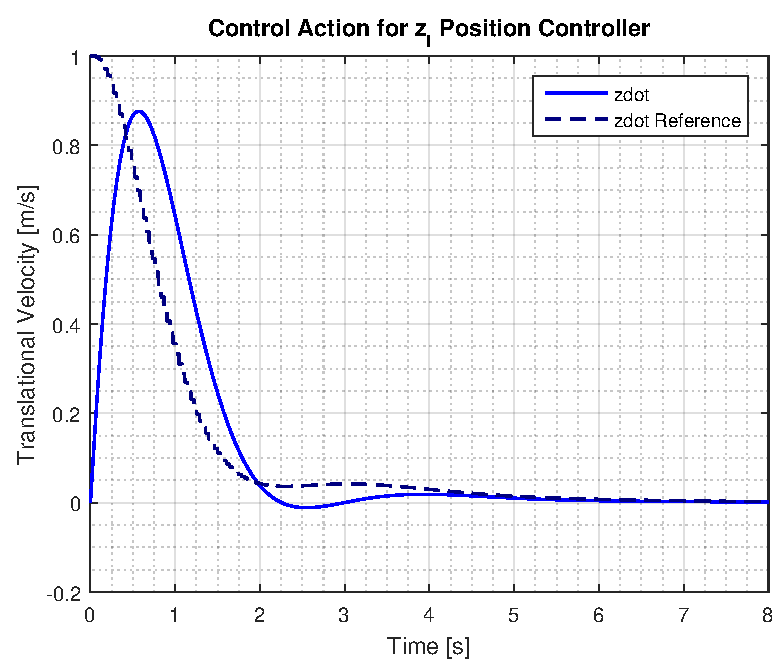
\includegraphics[scale=.45]{figures/positionControllerZAction}
            \centering
            \captionof{figure}{Control action imposed on the system by the z translational position controller, which is then realized by the velocity controller to achieve the position response seen in \autoref{fig:positionControllersZ}.}
            \label{fig:positionControllerZAction}
        \end{figure}
    \end{minipage}
\end{minipage}